\chapter{Les Clients}

\section{La page "Clients"}
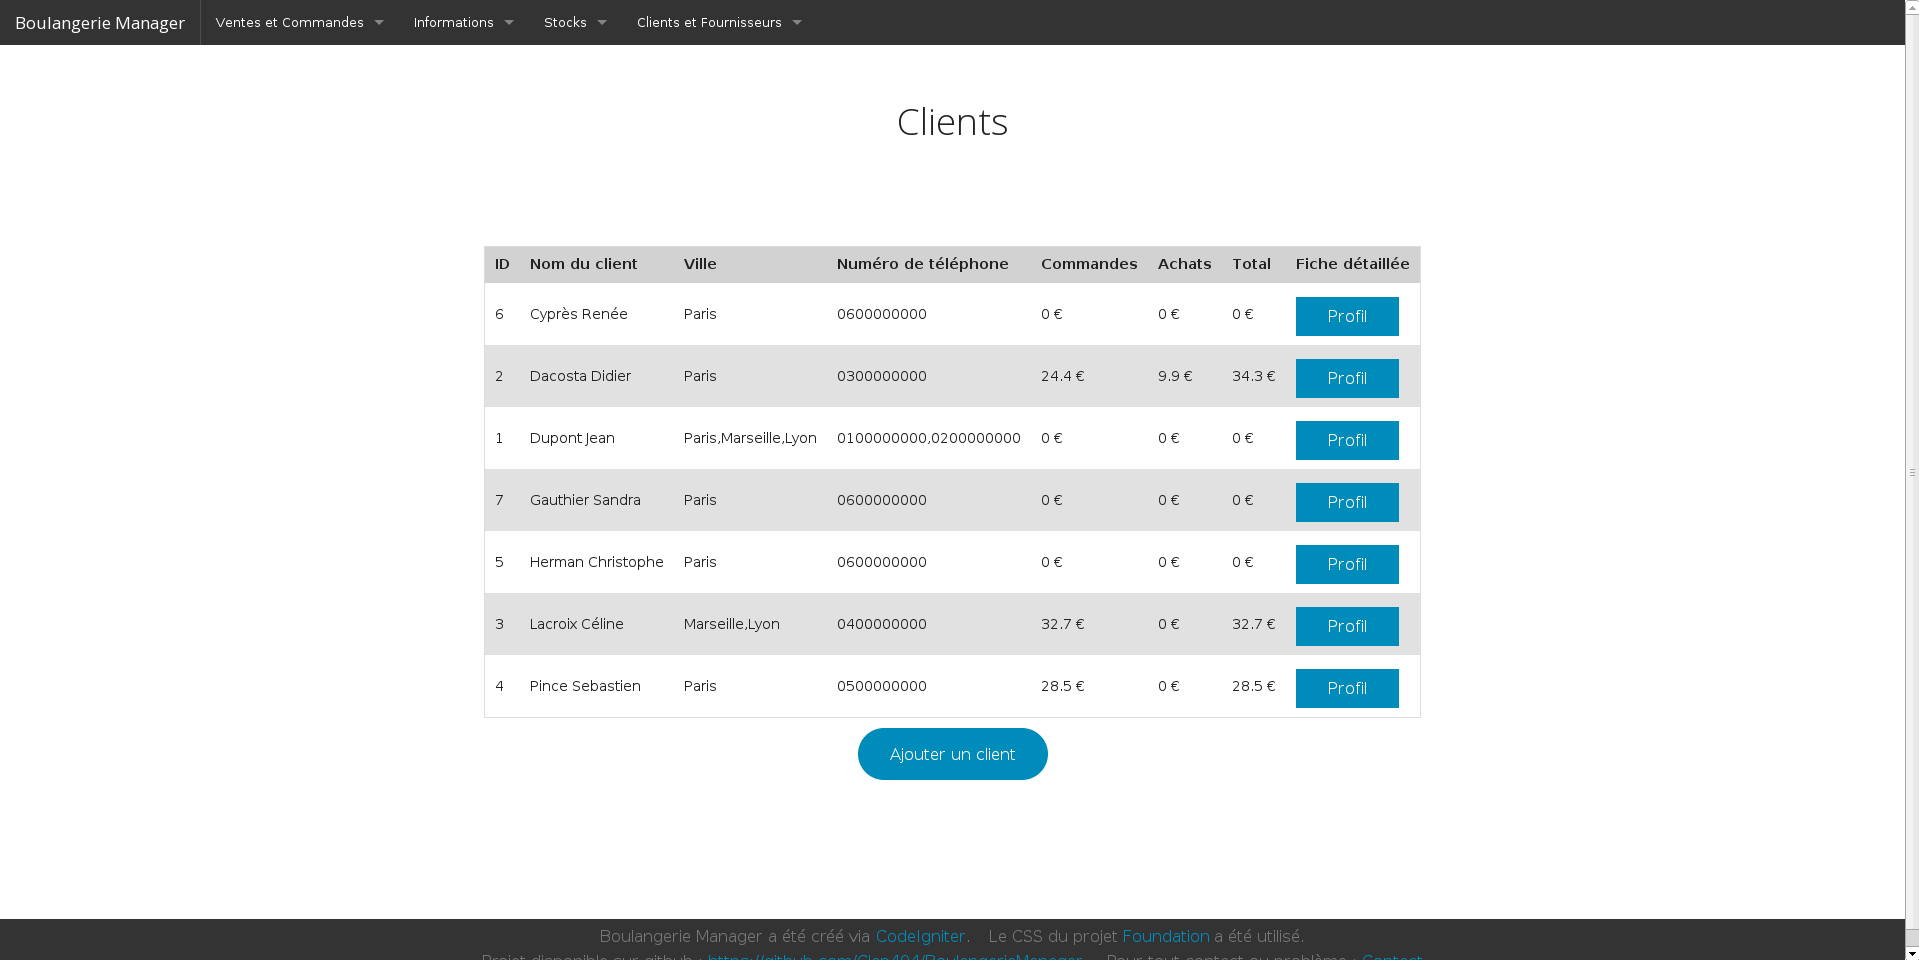
\includegraphics[scale=0.30]{client1.png}\\
Cette page liste les clients par ordre alphabétique. Pour chaque client, sont
affichés le nom et prénom, les villes de résidence, les numéros de téléphone, 
ainsi que les montants des commandes passées et des achats effectués, affichés
séparément puis sommés.

\paragraph{}
Le bouton "Profil" permet d'accéder à la fiche détaillée de chaque client.

\subsection{Ajout d'un client}
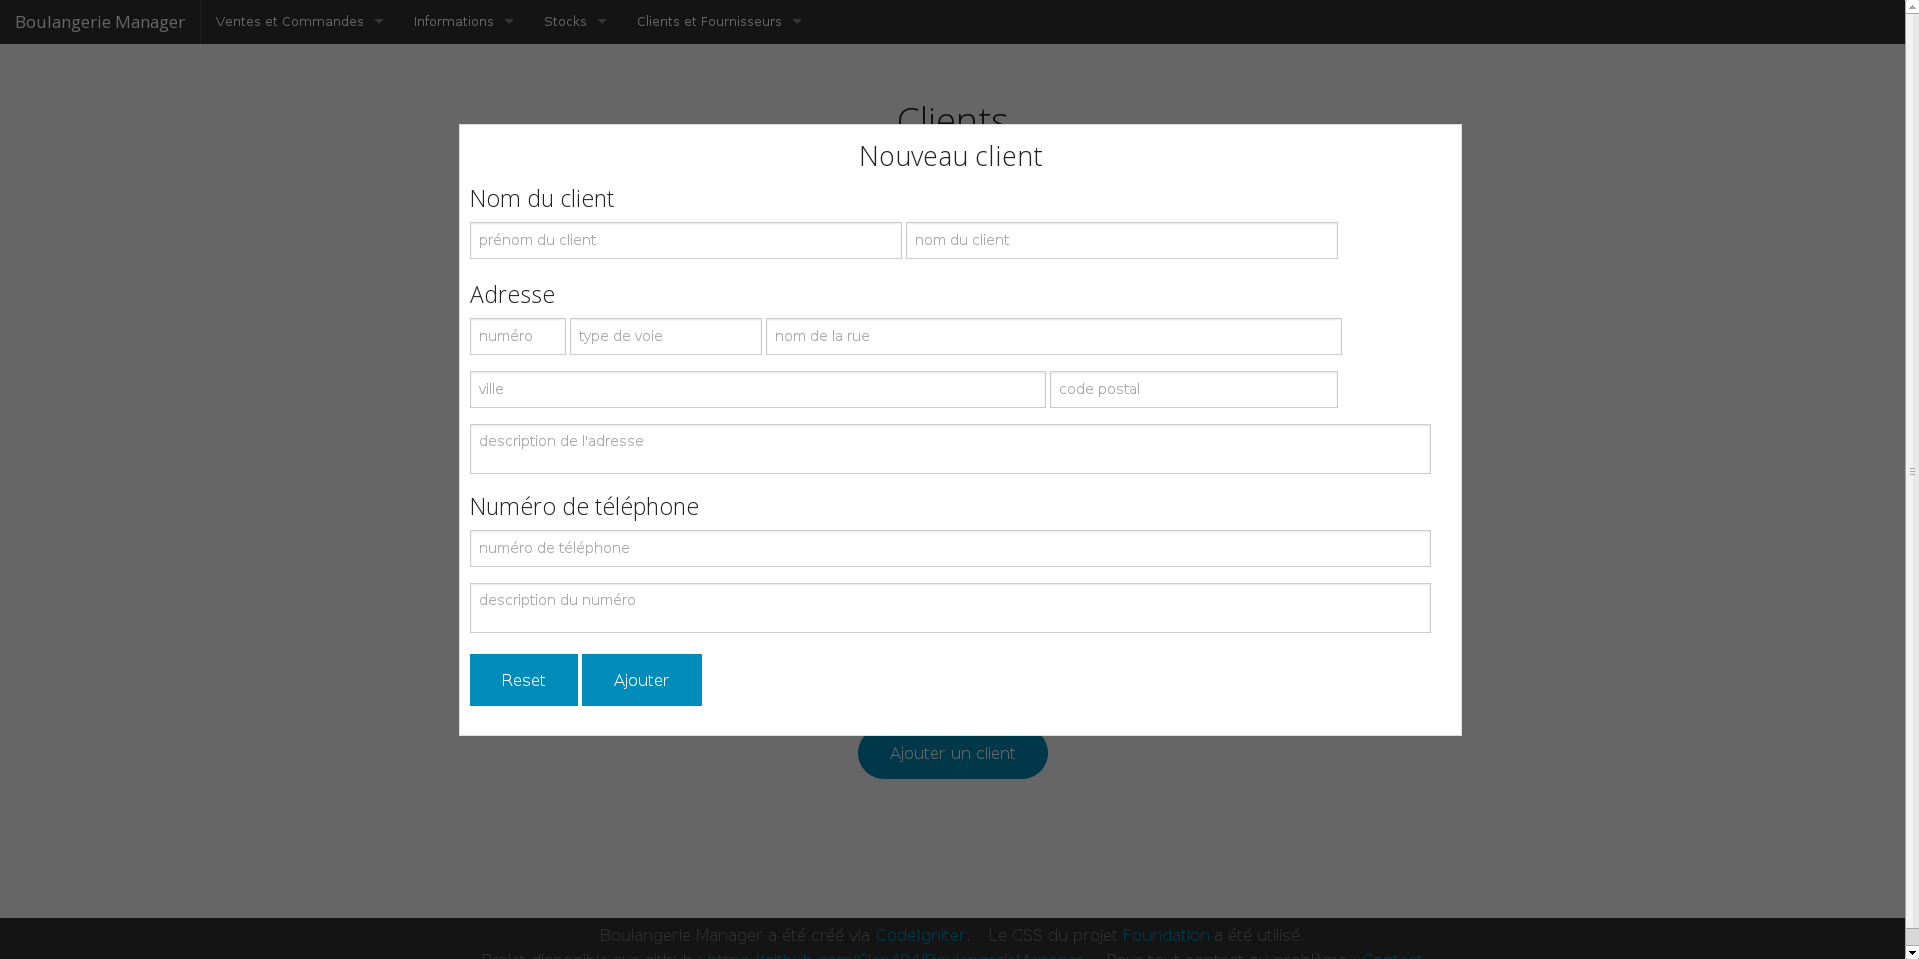
\includegraphics[scale=0.30]{client3.png}\\
Sur la page "Clients", la liste de clients est suivie d'un bouton
"Ajouter un client". Un clic sur ce bouton fait apparaître un formulaire au
premier plan. Entrez les informations demandées par le formulaire puis cliquez
sur "Ajouter" pour enregistrer le nouvel utilisateur. Si les données sont
ajoutées avec succès, le mot "Succès" s'affichera un bref instant à droite du
formulaire avant qu'il ne disparaisse.

\paragraph{}
Dans le cas où certaines informations
sont manquantes ou ne correspondent pas au type de donnée attendu, des messages
précisant les champs incorrects seront affichés à droite du formulaire; il sera
alors nécessaire de corriger les champs avant de soumettre à nouveau le
formulaire.

\paragraph{}
Le bouton "Reset" permet d'effacer le contenu de tous les champs. Un clic en
dehors du formulaire fermera celui-ci.

\subsection{Aide au remplissage}
Le formulaire d'ajout dispose d'une aide au remplissage pour certains champs :
un menu contextuel proposant des valeurs existant déjà en mémoire. Pour profiter
de l'aide au remplissage sur un champ, tapez la première lettre dans le champ
puis sélectionnez la valeur souhaitée dans le menu contextuel grâce aux touches
fléchées suivi d'un appui sur entrée pour valider.

\paragraph{}
Si le menu contextuel ne contient pas la valeur souhaitée, tapez les lettres
suivantes jusqu'à compléter votre saisie ou bien voir apparaître la valeur
désirée dans le menu contextuel.

\section{La page "Profil"}
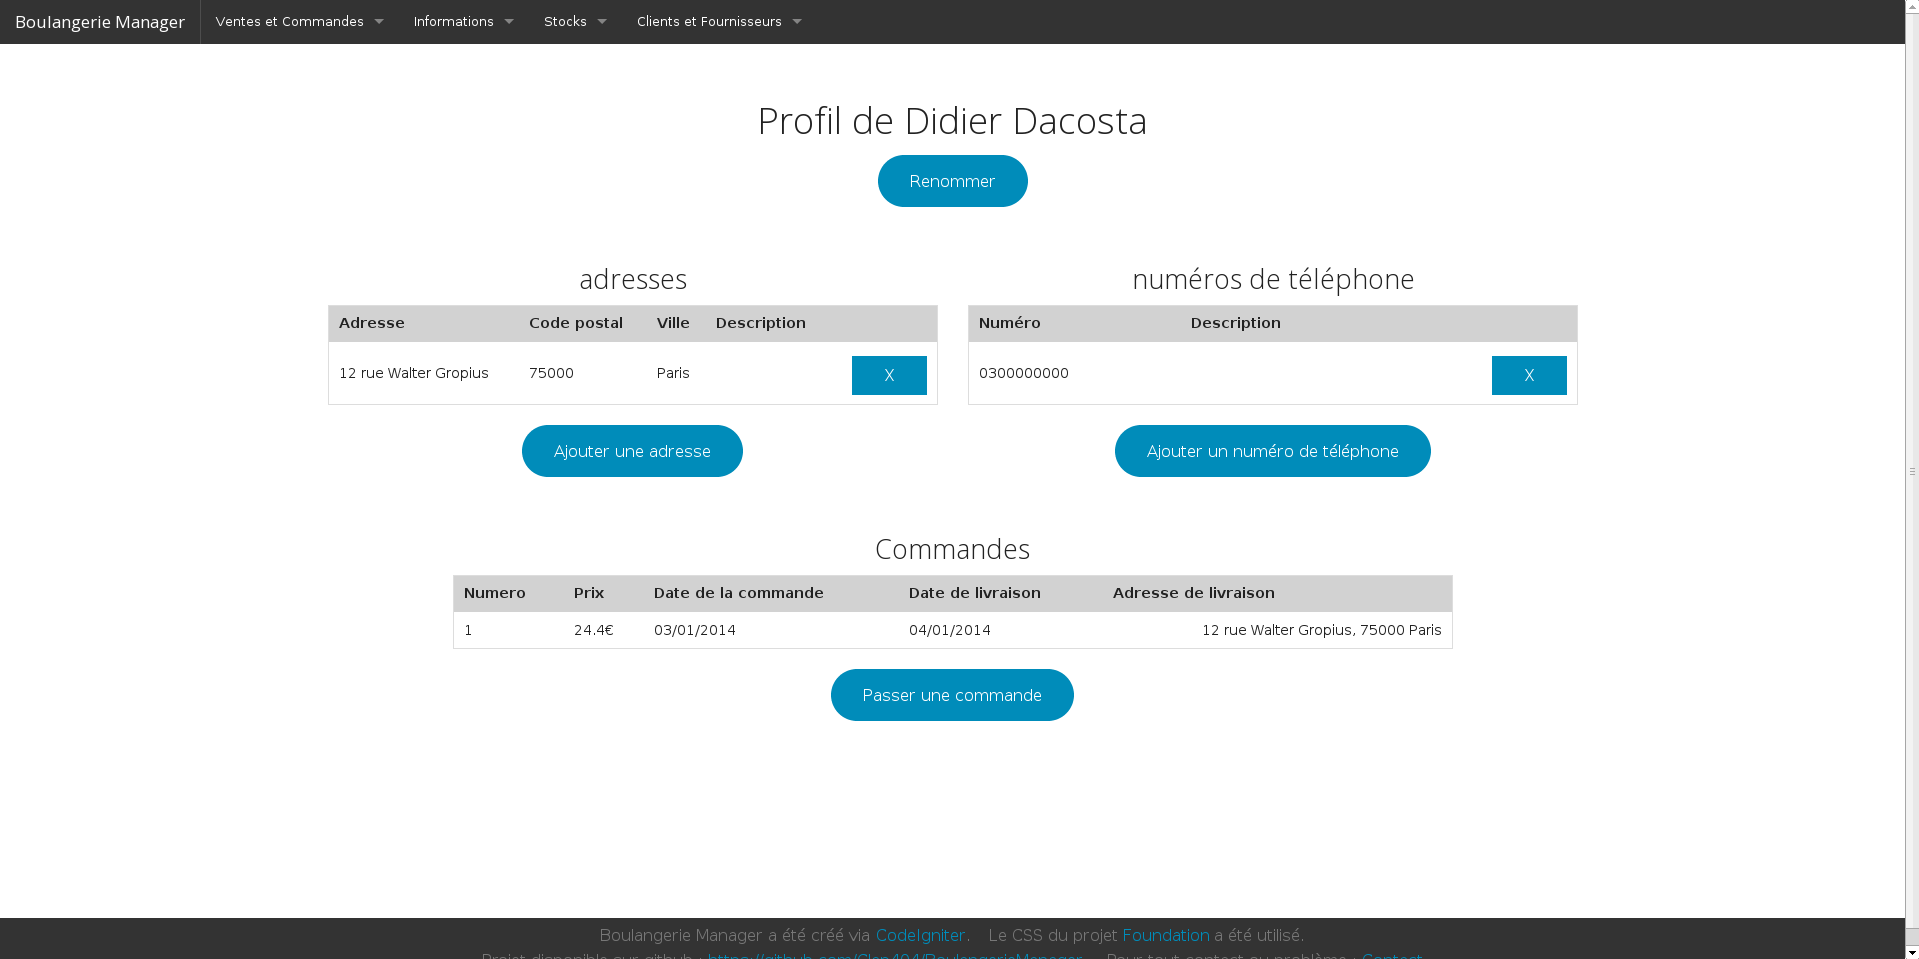
\includegraphics[scale=0.30]{client2.png}\\
La page de profil est composée de quatre champs d'information :

\begin{enumerate}
  \item Le nom du client
  \item Les adresses du client
  \item Les numéros de téléphone du client
  \item Les commandes effectuées par le client
\end{enumerate}

\subsection{Ajout d'informations sur les clients}
Chaque champ d'information est accompagné d'un bouton permettant l'ajout d'informations.
Un clic sur l'un de ces boutons fait apparaître le formulaire d'ajout
d'information associé.

\paragraph{}
Le bouton "Passer une commande" vous redirigera vers la page des commandes
tandis que les trois autres boutons feront apparaître un formulaire au premier
plan. Comme pour l'ajout d'un client, chaque formulaire possède un bouton "Reset"
qui efface toutes les valeurs entrées dans le formulaire sans valider et un
bouton "Ajouter" qui enregistre les données ou demande une rectification de
certaines zones de saisie si une erreur est trouvée.

\subsection{Suppression d'informations sur les clients}
Les lignes pouvant être supprimée possèdent
un bouton avec une croix. Un clic sur ce bouton supprime directement
l'information de la mémoire.

\paragraph{}
Les listes "Adresses" et "Numéros de téléphone" doivent toujours contenir au
moins une entrée. Par conséquent, le bouton de suppression de fonctionnera pas
si la liste ne contient plus qu'une entrée.
